% MATH 578 FINAL (F16)
% LUKE WUKMER

\documentclass[10pt]{article}

% note: some of these are extremely useful and i don't remember why :o
%\usepackage{savetrees} % disable custom geometry stuff if you do this
\usepackage{titling}    % contol over title & stuff
\usepackage{amsmath, amsthm, amssymb, amsfonts}
\usepackage{amsxtra, amscd, geometry, graphicx}
\usepackage{endnotes}
\usepackage{cancel}
\usepackage{wrapfig}    %inline figs
\usepackage{bm} %allows fancy stuff like bold greek in math mode
\usepackage{alltt}
\usepackage{enumerate} %more/easier control over lists, also see enumitem
%\usepackage[all,cmtip]{xypic}
\usepackage{mathrsfs}
\usepackage{listings} % code with syntax highlighting etc
\usepackage{caption}
\usepackage[raggedright]{sidecap} % side captions
\usepackage{tabu}     % more customizable tables
%\usepackage{subfigure}
%\usepackage{subcaption}
%\usepackage[pdftex]{hyperref}
%\usepackage[dvips,bookmarks,bookmarksopen,backref,colorlinks,linkcolor={blue},citecolor={blue},urlcolor={blue}](hyperref}

\graphicspath{ {./figs/} }

\usepackage{color}
\definecolor{mygreen}{rgb}{0,0.6,0}
\definecolor{mygray}{rgb}{0.5,0.5,0.5}
\definecolor{mymauve}{rgb}{0.58,0,0.82}

\lstset{ %
basicstyle=\ttfamily,        % the size of the fonts that are used for the code
%breakatwhitespace=false,         % sets if automatic breaks should only happen at whitespace
breaklines=false,                 % sets automatic line breaking
captionpos=t,                    % sets the caption-position to bottom
commentstyle=\color{mygray},    % comment styleh
%  deletekeywords={...},            % if you want to delete keywords from the given language
%  escapeinside={\%*}{*)},          % if you want to add LaTeX within your code
% extendedchars=true,              % lets you use non-ASCII characters; for 8-bits encodings only, does not work with UTF-8
frame=single,                      % adds a frame around the code
%keepspaces=false,                 % keeps spaces in text, useful for keeping indentation of code (possibly needs columns=flexible)
% columns=flexible,
  keywordstyle=\color{blue},       % keyword style
  fontadjust=true,
  language=Python,                 % the language of the code
%  otherkeywords={*,...},           % if you want to add more keywords to the set
  numbers=left,                    % where to put the line-numbers; possible values are (none, left, right)
 numbersep=5pt,                   % how far the line-numbers are from the code
numberstyle=\tiny\color{mygray}, % the style that is used for the line-numbers
%  rulecolor=\color{black},         % if not set, the frame-color may be changed on line-breaks within not-black text (e.g. comments (green here))
showspaces=false,                % show spaces everywhere adding particular underscores; it overrides 'showstringspaces'
showstringspaces=false,          % underline spaces within strings only
%  showtabs=false,                  % show tabs within strings adding particular underscores
%  stepnumber=2,                    % the step between two line-numbers. If it's 1, each line will be numbered
  stringstyle=\color{mymauve},     % string literal style
%  tabsize=2,                      % sets default tabsize to 2 spaces
title=\lstname                   % show the filename of files included with \lstinputlisting; also try caption instead of title
}
% change up the fonts (pick one only)
%\usepackage{times}%
%\usepackage{helvet}%
%\usepackage{palatino}%
%\usepackage{bookman}%
\usepackage{dejavu}


% These are italic.
% \theoremstyle{definition}

% These are normal (i.e. not italic).
\theoremstyle{definition}

%\newtheorem{prob}{Problem}[section]
\newtheorem{prob}{Problem}
\newtheorem*{prob*}{Problem}
\newtheorem*{soln*}{Solution}
\newtheorem{soln}{Solution}


% New Commands: Common Math Symbols
\providecommand{\R}{\mathbb{R}}%
\providecommand{\N}{\mathbb{N}}%
\providecommand{\Z}{{\mathbb{Z}}}%
\providecommand{\sph}{\mathbb{S}}%
\providecommand{\Q}{\mathbb{Q}}%
\providecommand{\C}{{\mathbb{C}}}%
\providecommand{\F}{\mathbb{F}}%
\providecommand{\quat}{\mathbb{H}}%

% haha, i originally forked this template from one provided by my abstract
% algebra TA (back in 2012 or something). probably don't need most of these,
% huh. 

% New Commands: Operators
%\providecommand{\Gal}{\operatorname{Gal}}%
%\providecommand{\GL}{\operatorname{GL}}%
%\providecommand{\card}{\operatorname{card}}%
%\providecommand{\coker}{\operatorname{coker}}%
%\providecommand{\id}{\operatorname{id}}%
%\providecommand{\im}{\operatorname{im}}%
%\providecommand{\diam}{{\rm diam}}%
%\providecommand{\aut}{\operatorname{Aut}}%
%\providecommand{\inn}{\operatorname{Inn}}%
%\providecommand{\out}{{\rm Out}}%
%\providecommand{\End}{{\rm End}}%
%\providecommand{\rad}{{\rm Rad}}%
\providecommand{\rk}{{\rm rank}}%
%\providecommand{\ord}{{\rm ord}}%
%\providecommand{\comp}{{\text{ $\scriptstyle \circ$ }}}%
\providecommand{\cl}[1]{\overline{#1}}%
\providecommand{\tr}{{\sf trace}}%
\providecommand{\spn}{{\rm span}}%

\renewcommand{\tilde}[1]{\widetilde{#1}}%
%\numberwithin{equation}{section}

% i like the squiggly ones more. add as needed

\renewcommand{\Psi}{\varPsi}

\newcommand*\rfrac[2]{{}^{#1}\!/_{#2}}

% a very fancy dot product \ip{f}{g}
\newcommand\ip[2]{ \left\langle {#1} , {#2} \right\rangle }

% "s.t." for math mode
\providecommand{\st}{\text{ s.t. }}

% \norm{f} and such, super useful
\newcommand{\norm}[1]{\left\lVert#1\right\rVert}

% determinant
%\newcommand{\det}[1]{\textsf{det}\left(#1\right)}

% jacobian
\providecommand{\J}{\textsf{J}}

% this makes the spacing between lines of font a little bigger
%\newcommand{\spacing}[1]{\renewcommand{\baselinestretch}{#1}\large\normalsize}
%\spacing{1.2}

\DeclareMathOperator*{\argmin}{arg\,min}
\DeclareMathOperator*{\argmax}{arg\,max}

\newcommand*\mcol[1]{\overset{\big\uparrow}{\underset{\big\downarrow}{#1}}}

% Makes the margin size a little smaller, i gots stuff to say
\geometry{letterpaper,margin=.8in}

% titling stuff (from package titling)
\posttitle{\par\end{center}}
\setlength{\droptitle}{-.5in}
% END PREAMBLE %%%%%%%%%%%%%%%%%%%%%%%%%
%%%%%%%%%%%%%%%%%%%%%%%%%%%%%%%%%%%%%%%%


\begin{document}

\title{Math 578 Final}
\author{Luke Wukmer}
\date{Fall 2016}
\maketitle \thispagestyle{empty} % remove the page number from the first page

\begin{section}{The Problem}
We use Multigrid-Preconditioned Conjugate Gradient Method (henceforth referred to as \textbf{MGCG}) to solve a particular problem:
\[
Ax=b
\]
where
\begin{equation}
A \in \R^{2^M \times 2^M} ,\quad A_{ij} = \begin{cases}
3 & \text{if}\quad j = i, \\
-1 & \text{if}\quad j = i \pm 1 \\
-1 & \text{if}\quad  j = N - i + 1, i \ne \frac{N}{2}, \frac{N}{2}+1
\end{cases},\\
\end{equation}
and b is a $N\times1$ normalized one vector.

We will compare two methods of preconditioning via multigrid, defined here:

\subsection{Scenario \#1}
In "scenario \#1" (referred to henceforth as \textbf{SC1}), we precondition via multigrid using the following interpolation matrix (between levels $l$ and $l-1$) (refer to equation \#2 in the project spec):

\begin{lstlisting}
def interpolation_matrix(M,L,el):
    """
    The interpolation matrix I_el between levels el and (el-1)
    INPUT:
    M -     refers to size of system 2^M x 2^M 
    L -     number of levels/grids
    el-     interpolate between el and el-1 

    OUTPUT:
    I_el    a 2^{ M + el - L } by 2^{M + el - (L + 1) }
            interpolation matrix
    """

    n = 2**(M + el - (L+1))

    # identity matrix but repeat each row twice
    # (equivalent to given system)
    return np.repeat(np.eye(n), 2, axis=0)
\end{lstlisting}
\clearpage
\subsection{Scenario \#2}
Scenario \#2, (\textbf{SC2}) is the same as the above, but we change precisely one level of interpolation: between the second and third finest levels. Refer to spec and the code below.
\begin{lstlisting}
def interpolation_matrix_2(M,L,el):
    """
    The interpolation matrix I_el between levels el and (el-1)
    for example if M = 2, this function would return
         array([[ 1.,  0.,  0.,  0.],
                [ 0.,  1.,  0.,  0.],
                [ 0.,  0.,  1.,  0.],
                [ 0.,  0.,  0.,  1.],
                [ 0.,  0.,  0.,  1.],
                [ 0.,  0.,  1.,  0.],
                [ 0.,  1.,  0.,  0.],
                [ 1.,  0.,  0.,  0.]])

    for the given question, this is only to be used for the
    (L-1) to (L-2)th level
    """
    if el != L-1:
        return interpolation_matrix(M,L,el)
    else:
        n = 2**(M-2)
        return np.concatenate((np.eye(n),np.flipud(np.eye(n))))

\end{lstlisting}
\end{section}
\begin{section}{Implementation}
\begin{subsection}{The V-cycle}
The following is a basic implementation of the multigrid "v-cycle." 
\begin{lstlisting}
def vcycle(l,b,e0, A, I, Lchol):
    
    omega = 2/3
    nu1 = 1
    # base case
    if l == 1:
        e_base = linalg.solve(Lchol.T,linalg.solve(Lchol,b))
        return e_base
    else:
        a = A[-(l-1)]
        i = I[-(l-1)]
        e = smooth(a, omega, nu1, b, e0)
        # compute and restrict error
        res = i.T @ (b - a@e)
        # correct error
        e = e + i @ vcycle(l-1,res, np.zeros_like(res), A,I,Lchol)
        # smooth nu1 times on a x = b with initial guess e
        e = smooth(a,omega,nu1,b,e)

    return e
\end{lstlisting}
\end{subsection}
\begin{subsection}{Smoothing function}
Here is the smoothing function. As described in the docstring,
this function was first tested for accuracy by applying it to a
$4\times4$ diagonally dominant system. This system was suggested
by the Wikipedia page for Jacobi iteration.

\begin{lstlisting}
def smooth(A, omega, nu, b, x0, tol=None):
    """
    smoothing function via ω-weighted Jacobi iteration
    this is also a standard iterative method on a
    diagonally dominant system

    AA = np.array([[10., -1., 2., 0.],
                   [-1., 11., -1., 3.],
                   [2., -1., 10., -1.],
                   [0.0, 3., -1., 8.]])

    bb = np.array([6., 25., -11., 15.])
    x00 = np.zeros_like(bb)
    ans = smooth(AA,1., 50, bb, x00)

    converges after 24 iterations
    
    if omega is changed to 2/3 in the above, converges in 35 iterations
    """
    if x0.ndim == 1:
        x0 = np.expand_dims(x0,-1)
    if b.ndim == 1:
        b = np.expand_dims(b,-1)
    
    x = x0.copy()
    D = np.diag(A) # diagonal of system (as a Nx1 vector)
    # must be same shape as b or will broadcast to a matrix under division
    D = D.reshape(x.shape)

    W = np.tril(A, k=-1) + np.triu(A,k=1) #deleted diagonal

    for i in range(nu):
        x = (1-omega)*x + ((omega*(b- (W@x))) / D)
        if tol is not None and np.allclose(b,A@x, 1e-12):
            break
    else:
        if tol is not None:
            print("Warning, did not converge within tolerance", tol)

    return x
    \end{lstlisting}
\end{subsection}
\clearpage
\subsection{MGCG (Full Method)}
\begin{lstlisting}
def mgcg(A, b, n_levels=0,interpolation_method=None, verbose=False):
    """
    Multigrid preconditioned Conjugate Gradient Method
    This solves the system Ax=b for a particular system A.
    
    if n_levels is 0 do unpreconditioned CG
    """
    M = int(np.log2(A.shape[0]))
    # check that A is actually a power of 2 (no strategy otherwise)
    N = A.shape[0]

    assert 2**M == N
    
    preconditioned =  (n_levels != 0 and interpolation_method is not None) 

    if preconditioned: 
        
        # build *all* interpolation matrices and store
        I = tuple((interpolation_method(M,n_levels,l)
                for l in range(n_levels,1,-1)))
        a = A
        A_levels = list() # store all systems
        for interp in I:
            A_levels.append(a) # append last system matrix

            # yer done if interp is 0x0 (only an issue if L is larger than M)
            if not interp.size:
                break

            a = interp.T @ (a @ interp)

        # now base_case
        A_1 = a
        A_levels = tuple(A_levels) # make static

        # you may check np.allclose(Lchol, linalg.cholesky(A_1,lower=True))
        Lchol, it_chol = cholesky(A_1)

        Minv = lambda b: vcycle(n_levels,b,np.zeros_like(b),A_levels,I,Lchol)    


    else:
        # if n_levels == 0 then do unpreconditioned CG
        # i.e. preconditioner is the identity
        Minv = lambda b: b

    pcg_sol, its = pcg(A,b, Minv, return_iterations=True, verbose=verbose)
    
    if preconditioned:
        return pcg_sol, its, A_levels, I
    else:
        return pcg_sol, its, A, None
\end{lstlisting}
\end{section}
\begin{section}{Results}
When the program \texttt{mgcg.py} is run by itself, the following output is generated. Here, \texttt{interpolation\_matrix} and \texttt{interpolation\_matrix\_2}
refer to PCG in scenario \#1 and \#2, respectively, while \texttt{None} refers to
unpreconditioned CG.
\begin{small}
\begin{verbatim}
____________________________________________________________
M= 11 L= 6
method: <function interpolation_matrix at 0x7f52b04bbc80>
	 65 iterations
	 time elapsed= 8.153933763504028
____________________________________________________________
____________________________________________________________
M= 11 L= 6
method: <function interpolation_matrix_2 at 0x7f52b04bbd08>
	 41 iterations
	 time elapsed= 4.9130401611328125
____________________________________________________________
____________________________________________________________
M= 11 L= 6
method: None
	 512 iterations
	 time elapsed= 3.9258689880371094
____________________________________________________________
____________________________________________________________
M= 12 L= 7
method: <function interpolation_matrix at 0x7f52b04bbc80>
	 99 iterations
	 time elapsed= 46.1121826171875
____________________________________________________________
____________________________________________________________
M= 12 L= 7
method: <function interpolation_matrix_2 at 0x7f52b04bbd08>
	 61 iterations
	 time elapsed= 28.609034299850464
____________________________________________________________
____________________________________________________________
M= 12 L= 7
method: None
	 1024 iterations
	 time elapsed= 29.122495651245117
____________________________________________________________
____________________________________________________________
M= 13 L= 8
method: <function interpolation_matrix at 0x7f52b04bbc80>
	 158 iterations
	 time elapsed= 258.28484988212585
____________________________________________________________
____________________________________________________________
M= 13 L= 8
method: <function interpolation_matrix_2 at 0x7f52b04bbd08>
	 87 iterations
	 time elapsed= 147.13387250900269
____________________________________________________________
____________________________________________________________
M= 13 L= 8
method: None
	 2048 iterations
	 time elapsed= 237.42299604415894
____________________________________________________________

\end{verbatim}
\end{small}
For clarity, these results are summarized in a table below.

\subsection{Calculation of A-multiplies in CG/PCG}
	A fairly straightforward implementation of preconditioned conjugate gradient method is given below.
	\begin{lstlisting}
	def pcg(A,b, Minv, tol=1e-8, x_init=None, return_iterations=False,
	        return_error=False, verbose=False):
	    """
	    preconditioned conjugate gradient method
	    solves Ax = b by preconditioning
	
	    INPUT:
	
	    A       - an NxN nd.array describing the system
	    b       - initial conditions (can be 1D-array or 2D row vector)
	    Minv    - preconditioner, which should be a function handle
	    tol     - stopping tolerance (returns sol if ||A*sol - b}||_2 < tol ) 
	              (optional) default is 1e-8
	    x_init  - initial guess (default is None, in which case the zero vector
	                is used)
	
	    return_iterations   (optional) return iteration count (default False)
	    return_error        (optional) return error (will be below tolerance
	                        if converged)
	
	    OUTPUT:
	    x           - solution (an Nx1 nd.array)
	    iterations  -(if return_iterations=True above) iterations to run
	    err         -(||A*sol-b|| of solution calculated error of residual
	    """
	
	    # make sure initial guess is a column vector ala matlab
	    if b.ndim == 1:
	        b = np.expand_dims(b,-1)
	    
	    if x_init is None:
	        x = np.zeros_like(b) # default to zero vector as initial guess
	    else:
	        x = x_init
	
	    tol *= norm(b)  # for stopping check (save some divisions)
	
	    r = b - A@x     # initial residual
	    z = Minv(r)     # residual of preconditioned system
	    p = z.copy()    # initial search direction
	    d = A@p         # initial A-projected search direction
	
	
	    for iterations in count(1):
	
	        alpha = np.vdot(r,z) / np.vdot(p,d)
	
	        x += alpha*p
	        r_new = r - alpha*d
	        
	        # equivalent to norm(b - A@x) / norm(b)
	        err = norm(r_new)
	
	        if verbose:
	            print(iterations, err, sep='\t| ')
	
	        if err <= tol:
	            break
	        
	        z_new = Minv(r_new)
	        beta = np.vdot(z_new,r_new) / np.vdot(r,z)
	
	        p = z_new + beta*p
	
	        d = A@p
	    
	        r = r_new
	        z = z_new
	
	
	        #if err <= tol:
	        #    break
	    
	    # return statement boogaloo
	    if return_iterations:
	
	        if return_error:
	            return x, iterations, err / norm(b)
	        else:
	            return x, iterations
	
	    elif return_error:
	        return x, err / norm(b)
	
	    else:
	        return x
	\end{lstlisting}
	
Careful counting of the above shows there is exactly one $A$-multiplication and one
$M^{-1}$-multiplication in initialization, and one of each during each iteration. By hypothesis, each $M^{-1}$ (which is a v-cycle) corresponds to 5 A-multiplies. Thus PCG requires $ 1+k + 5*(1+k) =$ \boxed{$6+6k$} $A$-multiplies for $k$ iterations. By this logic, we can see that CG will only require \boxed{1+k} $A$-multiplies, (since CG is just PCG where $M^-1$ is identity).

\subsection{Tables (Iteration Counts, Speedup Ratio, Work Ratio)}
\begin{table}[h]\Large
\begin{center}
\begin{tabular}{lc|c|c}
	            &  M = 11 	& M = 12 	& M = 13\ \\ \hline
CG				&  512 		& 1024 		& 2048  \\
PCG \#1        	& 65 		& 99 		& 158  \\
PCG \#2         & 41 		& 61 		& 87  \\
\end{tabular}
\caption{Iteration counts of CG \& PCG on our system}
\end{center}
\end{table}
So solving our system (1) with unpreconditioned CG converges in the worst case, the exact size of the system. Either preconditioner is a massive improvement. Preconditioner \#2 converges in fewer iterations than preconditioner \#1.

\begin{table}[h]\Large
\begin{center}
\begin{tabular}{lc|c|c}
			            &  M = 11 & M = 12 & M = 13\ \\ \hline
CG vs. PCG \#1        	& 7.877 & 10.343 & 12.962  \\
CG vs. PCG \#2          & 12.488 & 16.787 & 23.540  \\
\end{tabular}
\caption{Speedup ratios of CG \& PCG on our system (approximate)}
\end{center}
\end{table}

\begin{table}[h]\Large
\begin{center}
\begin{tabular}{lc|c|c}
	            &  M = 11 & M = 12 & M = 13\ \\ \hline
CG vs. PCG \#1         	& 1.295 & 1.708 & 2.148  \\
CG vs. PCG \#2         & 2.036 & 2.755 & 3.88  \\
\end{tabular}
\caption{Work ratios of CG \& PCG on the system (approximate)}
\end{center}
\end{table}

Our tables suggest that implementation \#2 is much more efficient than implementation \#1, especially considering the number of $A$-multiplications per v-cycle can be drastically reduced (see section below).
\end{section}

\clearpage
\begin{section}{The Bonus Question Answered}
\subsection{The Answer}
If MGCG is performed on the system $A$ (1) using the interpolation method \textbf{SC2}, the optimal choice of level-depth $L$ is \begin{huge}\textbf{exactly 3}\end{huge} for any size $M\ge3$. That is, the "standard" interpolation step in (SC1) is used to interpolate between $A_L \rightarrow A_{L-1}$ and $A_{L-2}\rightarrow A_{L-3} = A_{1}$, and the "special" interpolation method unique to \textbf{SC2} is performed once in between. There are two reasons why, and they are clearly seen from a visual depiction of the multigrid systems of A using scenario \#2.

Refer to \textbf{Figure 1}, which was generated with the code \texttt{bonus\_demo.py}. Here we see the four finest systems in the multigrid when $M=7, L=6$, although this result is obviously true for any choice of $M$.
\begin{figure}[p]
\begin{center}
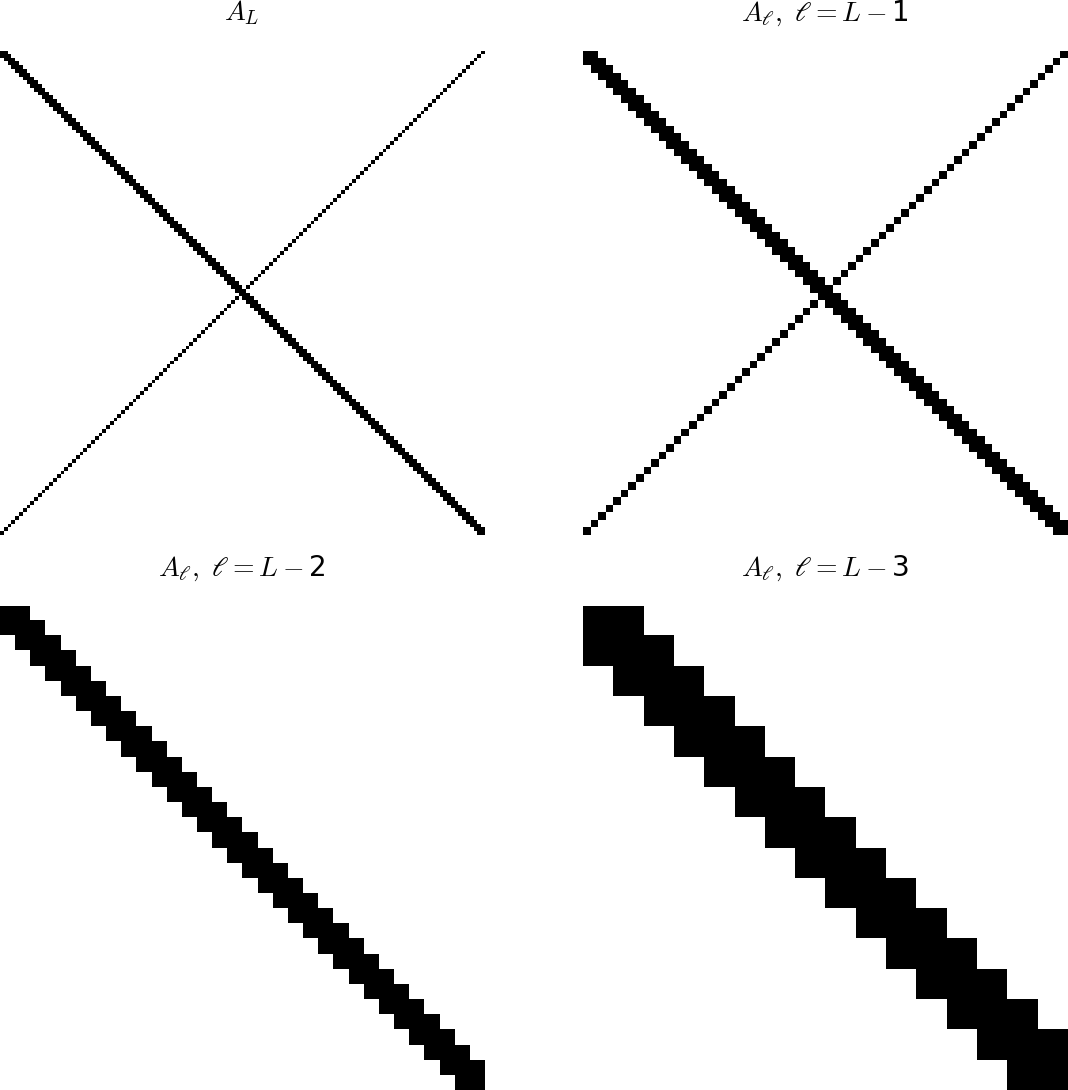
\includegraphics[width=0.8\linewidth]{scenario2_spy.png}
\caption{A look at the four finest levels of multigrid under \textbf{SC2}. After the second interpolation step, all subsequent levels are tridiagonal (and thus easily solved by Cholesky factorization)}
\end{center}
\end{figure}

\subsection{A loose justification}
The result is clear: applying the modified interpolation step between levels $A_{L-1}$ and $A_{L-2}$ converts the system from its original structure (with an antidiagonal) to a tridiagonal matrix, and all further interpolations preserve tridiagonality. Recalling that our goal in the V-cycle is to restrict the size of the system until we arrive at a system that is reasonable to solve directly, it makes sense that we should immediately solve such a system. There will be no additional benefit from successive restriction of the system once it is tridiagonal.

\lstinputlisting{bonus_demo.py}
\clearpage
\subsection{Empirical Support via Run times}
Of course, since performing the downscaling of the system A isn't computationally "free", we can directly see the superiority of choosing \textit{exactly} 3 levels. The following shows a session in \texttt{ipython}, where we perform the entire MGCG procedure on our system when $M=11$, iterating on the number of levels $L=1,2,\dots,9$. The average runtime over 3 runs is displayed for each L value. 

\begin{verbatim}
In [1]: from mgcg import * 
In [2]: M = 11
In [3]: A = make_system(M)
In [4]: b = make_initial_conditions(M)
In [5]: for L in range(1,10):
  ....:    %timeit mgcg(A,b,L,interpolation_matrix_2)
  ....:     
1 loop, best of 3: 2.65 s per loop
1 loop, best of 3: 1.86 s per loop
1 loop, best of 3: 1.48 s per loop	<-------------------------------
1 loop, best of 3: 2.79 s per loop
1 loop, best of 3: 3.96 s per loop
1 loop, best of 3: 4.99 s per loop
1 loop, best of 3: 6.84 s per loop
1 loop, best of 3: 7.58 s per loop
1 loop, best of 3: 7.9 s per loop
\end{verbatim}

These times are depicted in the graph below:
\begin{figure}[h]
\begin{center}
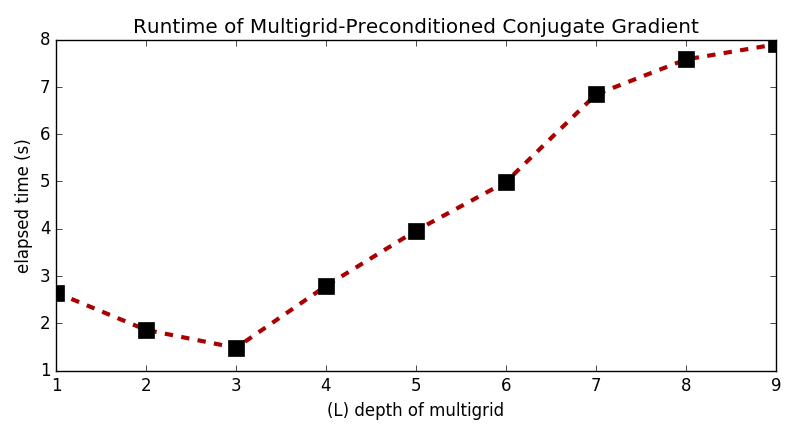
\includegraphics[width=0.8\linewidth]{runtimes.png}
\caption{Measuring run time of solving $Ax=b$ with MGCG when $M=11$, and varying $L$. Ran on a laptop using unoptimized code.}
\end{center}
\end{figure}
\pagebreak
\subsection{An alternative justification}
Figure 3 shows the effect of the preconditioners using both \textbf{SC1} and \textbf{SC2} on the initial condtions, as compared to the actual found solution of $Ax=b$ with system (1). Note the progress made by \textbf{SC2} after 3 levels is both more than *ever* achieved by \textbf{SC1} when we compare how the initial conditions are transformed.

This picture also gives a strong (yet loose and possibly fallacious) rationalization for the particular nature of the novel step in \textbf{SC2}: After a single round of restriction, the L-1 level restriction/interpolation step \textit{forces} the remaining solutions to be symmetric, with a crease in the middle (refer to implementation of $SC2$ in the spec and also this report). It just so happens that the particular solution to our $Ax=b$ is a very symmetrical solution, so (whatever the specifics), it is clear that the new step in \textbf{SC2} is exactly designed to exploit the \textit{expected} symmetry of the solution to $Ax=b$, whereas (SC1) does not take advantage of the symmetry.
\begin{figure}[h]
\begin{center}
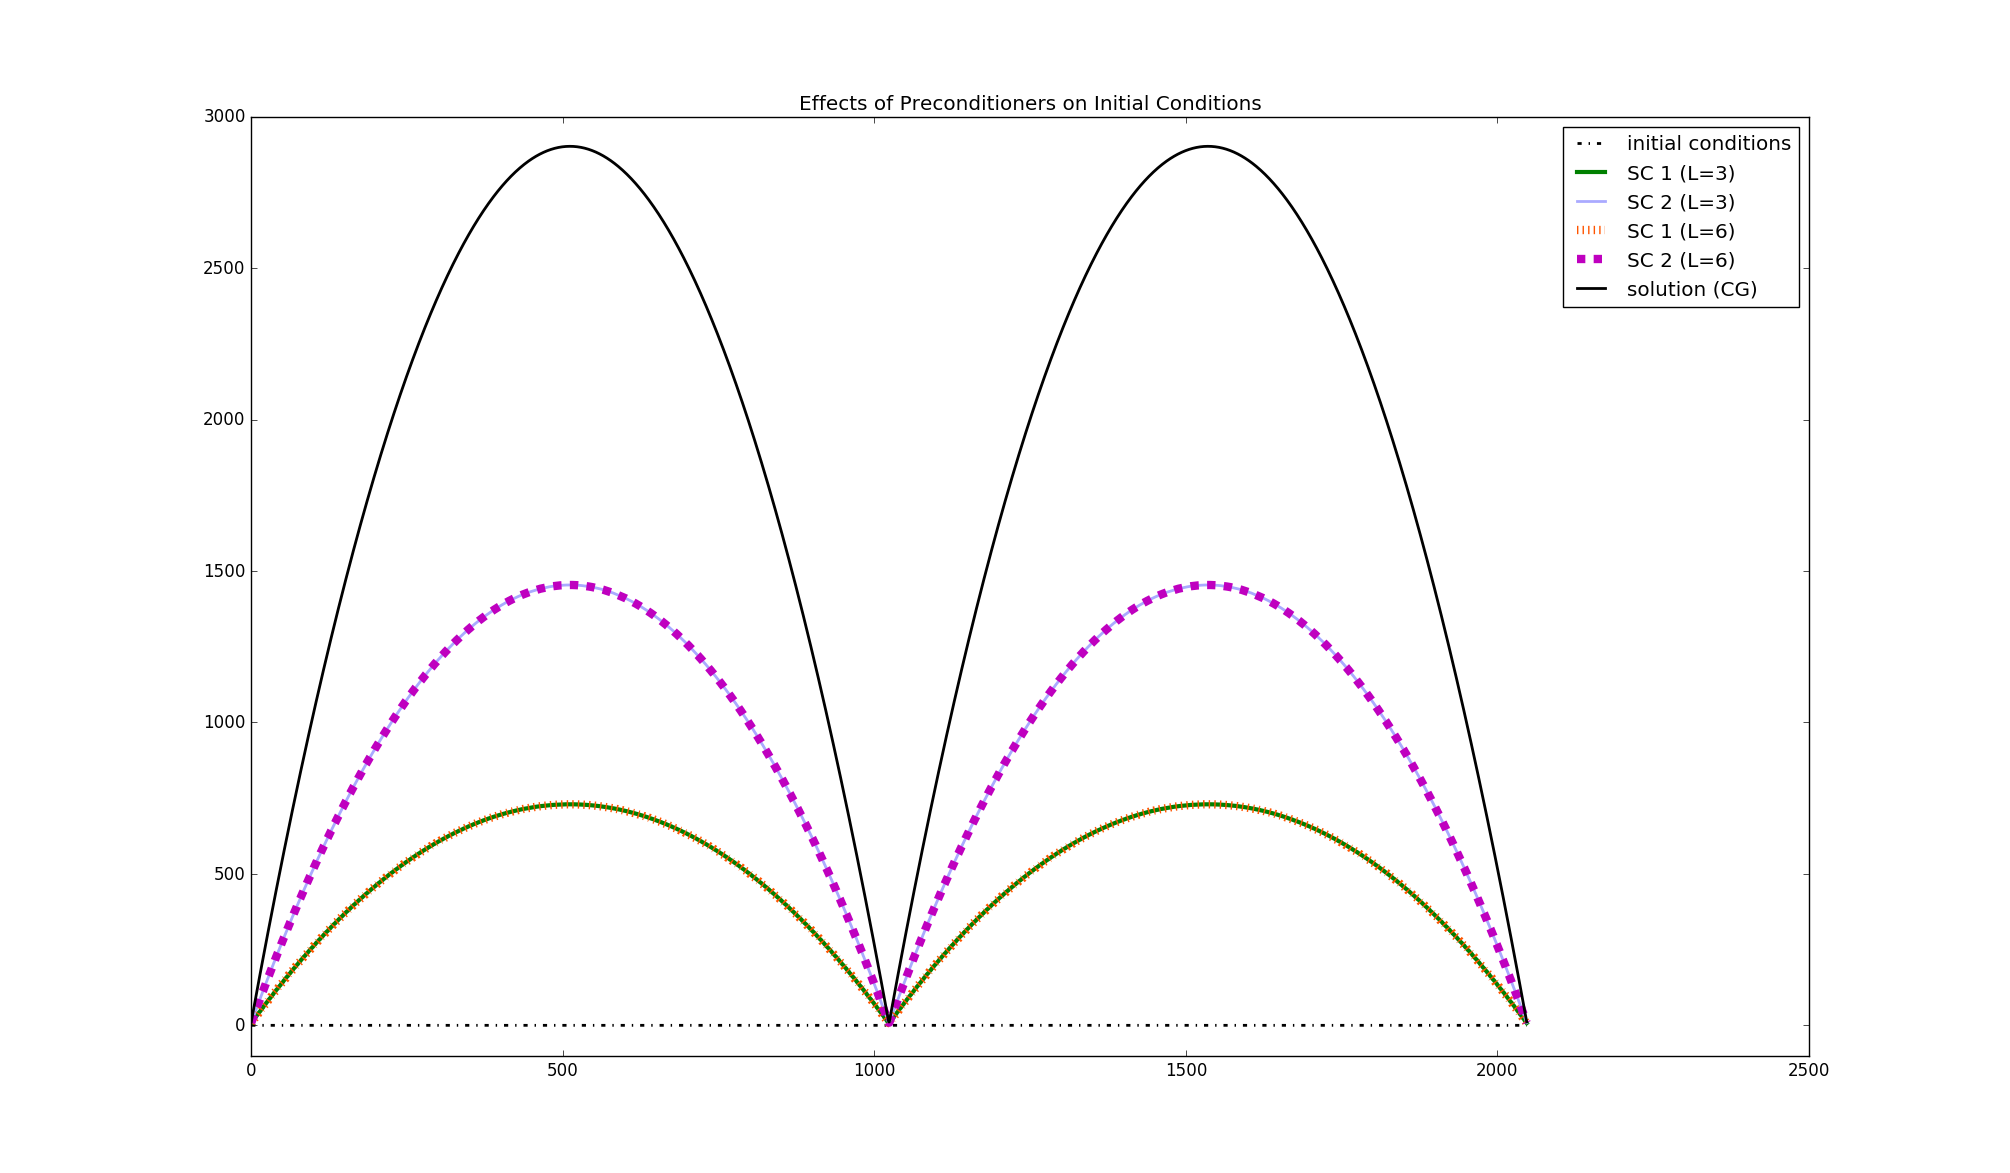
\includegraphics[width=\linewidth]{minv.png}
\caption{Measuring the proximity of a sample vector (the initial conditions and initial residual of PCG) to the eventual solution when $M=11$.}
\end{center}
\end{figure}
\end{section}
\end{document}

